\chapter{Testing}
\label{chap:testing}
To ensure that the platform works correctly and doesn't break any connectivity outside the remit of the automation platform, several tests were devised. Virtual Machines attached directly to hardware \gls{nic}s were used. These \gls{vm}s were connected as follows:

\begin{table}[htbp]
    \centering
    \begin{tabular}{@{} c c @{}}
        \toprule
        \textbf{Test VM}     & \textbf{Fabric Port} \\
        \midrule
        \texttt{1} & \texttt{FEX101/1}    \\
        \texttt{2} & \texttt{FEX102/1}    \\
        \texttt{3} & \texttt{FEX103/1}    \\
        \bottomrule
    \end{tabular}
    \caption{Test VM fabric connections}
\end{table}

This will allow for the testing of communication between different fabric nodes to determine if the \gls{aci} fabric has been provisioned correctly. Access to the internet from the test VMs will also be tested to ensure that the virtual router has been provisioned correctly. Connectivity to the project's terminal servers will also be tested from the test VMs.
The automation platform was setup as follows:

\begin{table}[htbp]
    \centering
    \begin{tabular}{@{} c c c @{}}
        \toprule
        \textbf{Rack}     & \textbf{Fabric Node} & \textbf{Terminal Server} \\
        \midrule
        \texttt{1} & \texttt{FEX101} & \texttt{TS-1}    \\
        \texttt{2} & \texttt{FEX102} & \texttt{TS-2}  \\
        \texttt{3} & \texttt{FEX103} &   \\
        \bottomrule
    \end{tabular}
    \caption{Rack to Fabric Node and Terminal Server mapping}
\end{table}


\subsection{Project Communication}
A new project was created with racks 1 and 2 being selected as members. Figure \ref{fig:test-project-1} shows the resulting project.

\begin{figure}[H]
    \centering
    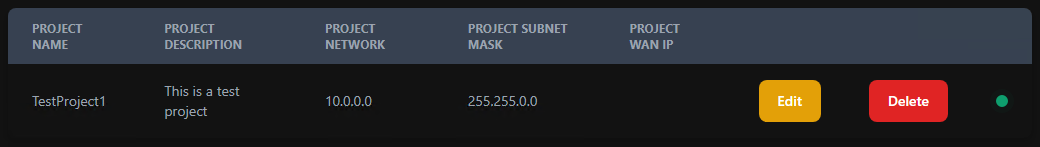
\includegraphics[scale=0.8]{images/test-project-1.png}
    \caption{Test Project 1 created successfully}
    \label{fig:test-project-1}
\end{figure}

As can be seen, the project has been allocated a subnet of 10.0.0.0/16. This can be used to set IP addresses on the 2 test \gls{vm}s. The IP addresses of 10.0.1.1 and 10.0.1.2 were chosen respectively. After assigning the IP addresses, the test \gls{vm}s were able to ping each other. Figures \ref{fig:test-project-1-ping-1} and \ref{fig:test-project-1-ping-2} shows the successful ping test, showing that the \gls{aci} fabric is being provisioned correctly.

\begin{figure}[H]
    \centering
    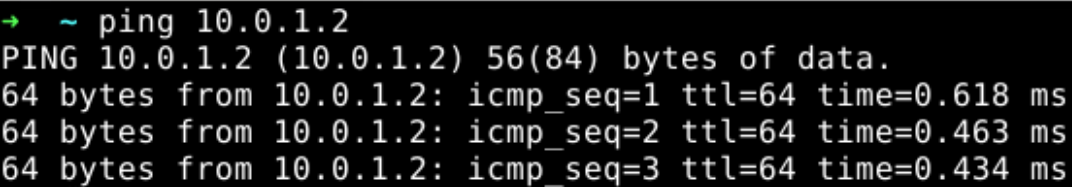
\includegraphics[scale=0.7]{images/test-project-1-ping.png}
    \caption{Test VM 1 pinging Test VM 2}
    \label{fig:test-project-1-ping-1}
\end{figure}

\begin{figure}[H]
    \centering
    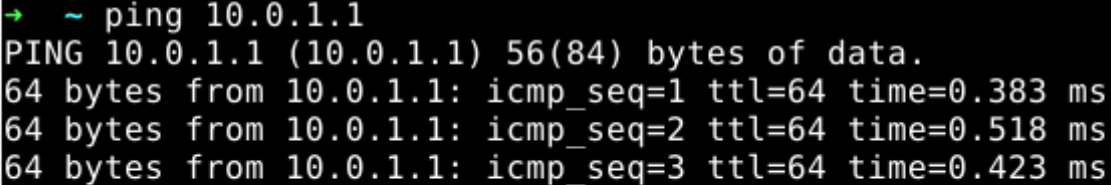
\includegraphics[scale=0.7]{images/test-project-1-ping-2.png}
    \caption{Test VM 2 pinging Test VM 1}
    \label{fig:test-project-1-ping-2}
\end{figure}

The next test was to ping the internet from the test \gls{vm}s. This was done by pinging the IP address of both Cloudflare and Google DNS, which is shown in figure \ref{fig:test-project-1-ping-internet}. This shows that the virtual router is being provisioned correctly.

\begin{figure}[H]
    \centering
    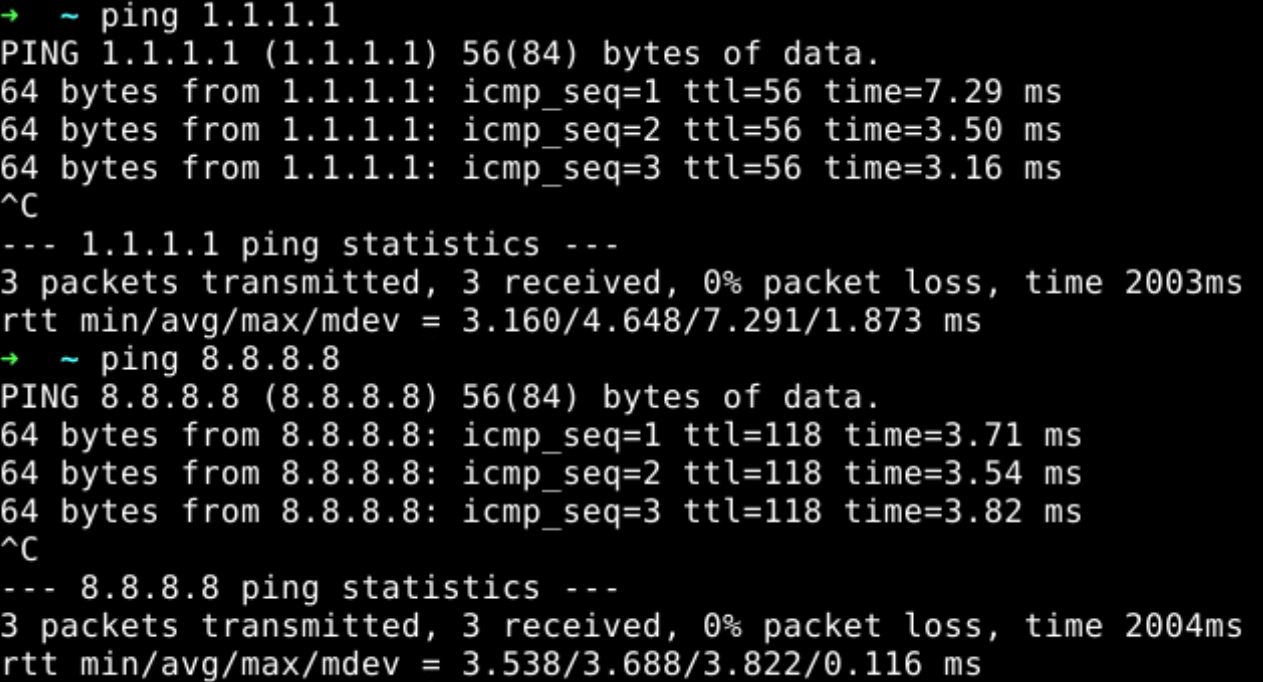
\includegraphics[scale=0.5]{images/test-project-1-ping-internet.png}
    \caption{Test VM 1 pinging the internet}
    \label{fig:test-project-1-ping-internet}
\end{figure}